\clearpage
\subsection{Record}
\hrulefill

1. Create a  Player Record Type and  show the details of a player.

\begin{lstlisting}[caption={ Query 1},label={lst:q-1}]
    DECLARE
    TYPE player_rec IS RECORD (
        player_id INT,
        player_name VARCHAR2(100),
        player_email VARCHAR2(100)
    );
    p_info player_rec;
BEGIN
    SELECT Player_ID, Player_Name, Player_Email
    INTO p_info
    FROM Player
    WHERE Player_ID = 1;
    DBMS_OUTPUT.PUT_LINE('Player ID: ' || p_info.player_id);
    DBMS_OUTPUT.PUT_LINE('Player Name: ' || p_info.player_name);
    DBMS_OUTPUT.PUT_LINE('Player Email: ' || p_info.player_email);
END;
/
\end{lstlisting}
\begin{figure}[H]
    \centering
    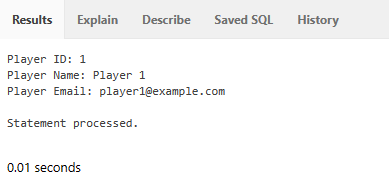
\includegraphics[width=0.5\textwidth]{images/plsql/record/Players Record.png}
    \caption{Result of Query 1}
\end{figure}
% Team Record Type

2. Create a Team Record Type and show the details of a team.
\begin{lstlisting}[caption={ Query 2},label={lst:q-2}]
    DECLARE
    TYPE team_rec IS RECORD (
        team_id INT,
        team_name VARCHAR2(100),
        team_country VARCHAR2(100)
    );
    t_info team_rec;
BEGIN
    SELECT Team_ID, Team_Name, Team_Country
    INTO t_info
    FROM Team
    WHERE Team_ID = 1;
    DBMS_OUTPUT.PUT_LINE('Team ID: ' || t_info.team_id);
    DBMS_OUTPUT.PUT_LINE('Team Name: ' || t_info.team_name);
    DBMS_OUTPUT.PUT_LINE('Team Country: ' || t_info.team_country);
END;
/

\end{lstlisting}
\clearpage
\begin{figure}[H]
    \centering
    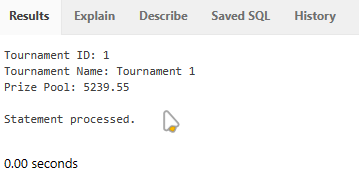
\includegraphics[width=0.5\textwidth]{images/plsql/record/Tournament Record Type.png}
    \caption{Result of Query 2}
\end{figure}

%Tournament Record Type
3. Create a Tournament Record Type and show the details of a tournament.

\begin{lstlisting}[caption={ Query 3},label={lst:q-3}]
    DECLARE
    TYPE tournament_rec IS RECORD (
        tournament_id INT,
        tournament_name VARCHAR2(100),
        prize_pool DECIMAL(10, 2)
    );
    t_info tournament_rec;
BEGIN
    SELECT Tournament_ID, Tournament_Name, Tournament_Prize_Pool
    INTO t_info
    FROM Tournament
    WHERE Tournament_ID = 1;
    DBMS_OUTPUT.PUT_LINE('Tournament ID: ' || t_info.tournament_id);
    DBMS_OUTPUT.PUT_LINE('Tournament Name: ' || t_info.tournament_name);
    DBMS_OUTPUT.PUT_LINE('Prize Pool: ' || t_info.prize_pool);
END;
/
\end{lstlisting}

\begin{figure}[H]
    \centering
    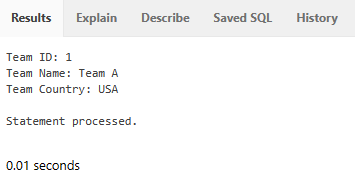
\includegraphics[width=0.5\textwidth]{images/plsql/record/Team Record Type.png}
    \caption{Result of Query 3}
\end{figure}